\scanpage{12}

% ll. 1–2
\mspage{\textcircled{10}}
De plus, on trouve ceci :

Considérons les \deleted{diagrammes}\inserted{graphes} suivants

% upper half, graph and count columns
\diagram{\scriptsize\setlength{\arraycolsep}{2pt}\(\displaystyle\begin{array}{clll|l}
&D_0=\varnothing&&&1\\
\cap&\text{\textcircled{$D_1$}}=&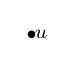
\begin{tikzpicture}[x=.65cm,y=.57cm,baseline=-.4ex,every node/.style={font=\scriptsize,inner sep=.9pt}]
\fill (0,0) circle (1.4pt) node[right] {$u$};
\end{tikzpicture}&\text{pt}&27=3^3.\\
\cap&D_2=&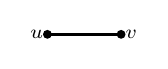
\begin{tikzpicture}[x=.65cm,y=.57cm,baseline=-.4ex,every node/.style={font=\scriptsize,inner sep=.9pt}]
\draw[very thick] (0,0) node[left] {$u$}--(1.44,0) node[right] {$v$};\fill (0,0) circle(1.6pt) (1.44,0) circle(1.6pt);
\end{tikzpicture}&\text{arête}&27.10=2.3^3.5=270\\
\cap&\text{\textcircled{$D_3$}}=&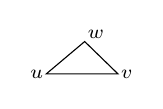
\begin{tikzpicture}[x=.65cm,y=.57cm,baseline=-.4ex,every node/.style={font=\scriptsize,inner sep=.9pt}]
\draw (0,0) node[left] {$u$} -- (.75,.72) node[above right] {$w$} -- (1.4,0) node[right] {$v$} -- cycle;
\end{tikzpicture}&\text{triangle}&27.10.1=2.3^3.5=270\\
\cap&D_4=&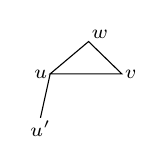
\begin{tikzpicture}[x=.65cm,y=.57cm,baseline=-.4ex,every node/.style={font=\scriptsize,inner sep=.9pt}]
\draw (0,0) node[left] {$u$} -- (.75,.72) node[above right] {$w$} -- (1.4,0) node[right] {$v$} -- cycle;\draw (0,0)--(-.19,-.98) node[below] {$u'$};
\end{tikzpicture}&\text{\deleted{triangle}\inserted{balai}.}&27.10.1.8=2^4.3^3.5=2160\\
\cap&D_5=&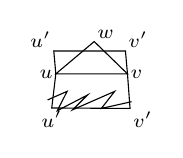
\begin{tikzpicture}[x=.65cm,y=.57cm,baseline=-.4ex,every node/.style={font=\scriptsize,inner sep=.9pt}]
\draw (0,0) node[left] {$u$} -- (.75,.72) node[above right] {$w$} -- (1.4,0) node[right] {$v$} -- cycle;\draw (0,0)--(-.04,.51) node[above left] {$u'$} -- (1.36,.51) node[above right] {$v'$} -- (1.4,0);
\draw (0,0)--(-.08,-.76) node[below] {$u'$}--(1.45,-.77) node[below right] {$v'$}--(1.4,0);
\draw (-.16,-.58)--(.22,-.39)--(.03,-.82)--(.62,-.47)--(.33,-.80)--(1.15,-.39)--(.89,-.77)--(1.48,-.62);
\end{tikzpicture}&\text{préprisme (triangulaire)}&27.10.1.8.4=2^6.3^3.5=8640\\
\cap&D_6=&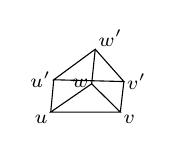
\begin{tikzpicture}[x=.65cm,y=.57cm,baseline=-.4ex,every node/.style={font=\scriptsize,inner sep=.9pt}]
\draw (0,0) node[below left] {$u$} -- (.8,.63) node[left] {$w$} -- (1.36,0) node[below right] {$v$} -- cycle;
\draw (.06,.72) node[left] {$u'$} -- (.87,1.4) node[above right] {$w'$} -- (1.43,.68) node[right] {$v'$} -- cycle;
\draw (0,0)--(.06,.72) (.8,.63)--(.87,1.4) (1.36,0)--(1.43,.68);
\end{tikzpicture}&\text{prisme (triangulaire)}&27.10.1.8.4.1=2^6.3^3.5=8640\\
\cap&\substack{\deleted{\unsure{D_7}}=\\\text{\textcircled{$D_7$}}}&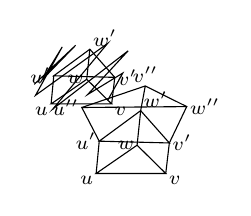
\begin{tikzpicture}[x=.65cm,y=.57cm,baseline=-.4ex,every node/.style={font=\scriptsize,inner sep=.9pt}]
\begin{scope}[shift={(-.88,1.55)},scale=.87]\draw (0,0) node[below left] {$u$} -- (.8,.63) node[left] {$w$} -- (1.36,0) node[below right] {$v$} -- cycle;
\draw (.06,.72) node[left] {$u'$} -- (.87,1.4) node[above right] {$w'$} -- (1.43,.68) node[right] {$v'$} -- cycle;
\draw (0,0)--(.06,.72) (.8,.63)--(.87,1.4) (1.36,0)--(1.43,.68);
\draw (-.38,.5)--(.55,1.5)--(-.20,.62)--(.25,1.46)--(-.35,.22)--(1.27,1.55)--(.04,-.13)--(1.73,1.36)--(.82,.24)--(1.61,.79)--(1.27,.09);\end{scope}
\draw (0,0) node[below left] {$u$} -- (.8,.63) node[left] {$w$} -- (1.36,0) node[below right] {$v$} -- cycle;
\draw (.06,.72) node[left] {$u'$} -- (.87,1.4) node[above right] {$w'$} -- (1.43,.68) node[right] {$v'$} -- cycle;
\draw (0,0)--(.06,.72) (.8,.63)--(.87,1.4) (1.36,0)--(1.43,.68);
\draw (.06,.72)--(-.28,1.47) node[left] {$u''$} -- (1.77,1.49) node[right] {$w''$} -- (1.43,.68);
\draw (-.28,1.47)--(.96,1.95) node[above] {$v''$} -- (1.77,1.49) (.96,1.95)--(.87,1.4);
\end{tikzpicture}&\text{bitriangle}&27.10.1.8.4.1.1=2^6.3^3.5=8640
\end{array}\)}

% ll. 11–12
Soit $\inserted{\mathrm{Pl}_i=}\mathrm{Pl}(D_i,C)$ l'ens des plongements \inserted{(``pleins'')} de $D_i$ dans $C$, $W=\operatorname{Aut} C$, $G_i=\operatorname{Aut}D_i$. Alors

% l. 13
\unsure{b)|c)|\deleted{b)}c)} Les $\mathrm{Pl}(D_i,C)$ sont des espaces homogènes (non vides) sous $G$

% ll. 14–16
a) Les morphismes $\mathrm{Pl}(D_{i+1},C)\mathbin{-}\mathrm{Pl}(D_i,C)$ $(0\leq i\leq6)$ transposés des inclusions $D_i\subset D_{i+1}$ sont surjectifs Ce sont des rev. d'ordres respectifs $27,10,1,8,4,1,1$

% ll. 17–18
b) (Par conséquent) les cardinaux des $\mathrm{Pl}_i$ sont les nbs marqués dans la colonne de droite.

% ll. 18–21
c) Par suite le \unsure{cardinal|cardinalx|cardinaux} \deleted{\unsure{des}} de l'ens \inserted{$\operatorname{Conf}_{D_i}(C)$} des sous-graphes \inserted{pleins} de $C$ \deleted{$\operatorname{Conf}_{D_i}(C)$} de type $D_i$ (s'identifiant à $\mathrm{Pl}_i/G_i$) est donné par $\operatorname{card}\mathrm{Pl}_i/\operatorname{card}G_i$, qui est

% left of assertions into bottom margin
\figure{\begin{tikzpicture}[x=.7cm,y=.48cm]
\draw[->] (1,6.7) .. controls (-.2,4.7) and (.16,2.6) .. (.35,2.2) .. controls (.6,-1) and (.52,-4.8) .. (1.05,-5.1);
\draw[->] (.26,3.38)..controls (.32,2.73) and (.52,2.26)..(1.11,2.18);
\end{tikzpicture}}

% bottom table, rows D0–D7
\diagram{\scriptsize\setlength{\arraycolsep}{2pt}\(\displaystyle\begin{array}{llcll}
\operatorname{Conf}_{D_0}\ {-}&1&--&\operatorname{Aut}D_0&e\\
\operatorname{Conf}_{D_1}&27&--&\operatorname{Aut}D_1&e\\
\operatorname{Conf}_{D_2}&27.10:2=135&---&\operatorname{Aut}D_2&\unsure{\mathfrak S|\mathcal S}_2\\
\operatorname{Conf}_{D_3}&27.10.1:6=45&--&\operatorname{Aut}D_3&\mathfrak S_3\\
\operatorname{Conf}_{D_4}&27.10.1.8:2=2^3.3^3.5=1080&--&\operatorname{Aut}D_4&\mathfrak S_2\\
\operatorname{Conf}_{D_5}&27.10.1.8.4:2=2^5\,3^3\,5=4320&--&\operatorname{Aut}D_5&\mathfrak S_2\\
\operatorname{Conf}_{D_6}&27.10.1.8.4.1:12=2^4\,3^2\,5=720&--&\operatorname{Aut}D_6&\mathfrak S_2\times\mathfrak S_3\\
\operatorname{Conf}_{D_7}&27.10.1.8.4.1.1:72=2^{3}.3.5=120&\cdots-&\operatorname{Aut}D_7&\unsure{\mathfrak S_2.(\mathfrak S_3\times\mathfrak S_3)}
\end{array}\)}
% archive sheet number: 11
